%%%%%%%%%%%%%%%%%%%%%%%%%%%%%%%%%%%%%%%%%

\chapter{Ultracold neutrons}\label{chap:UCN}

%%%%%%%%%%%%%%%%%%%%%%%%%%%%%%%%%%%%%%%%%

Ultracold neutron(s) (\ucn) are neutrons of very low kinetic energy ($\lesssim \qty{300}{\nano\eV}$) that have a number of convenient properties useful in experiments involving fundamental physics. Modern nEDM experiments are performed almost exclusively using UCN \cite{BAK06, SER15, ABE20} (an alternative is proposed in Ref.~\cite{PIE13}). Depending on the optical potential (Sec.~\ref{sec:ucn_matter_int}), \ucn may be contained at all angles of incidence by material bottles. They are also of low enough energies that they may be influenced by gravitational and magnetic potentials (Sec.~\ref{sec:ucn_grav_em}). Due to the ease of manipulation and transport, \ucn can be moved away from the production source, where backgrounds are typically high, into shielded environments where backgrounds may be controlled. \ucn are easy to polarize, and their polarization is easily measured (Sec.~\ref{sec:ucn_polarizers}). Neutrons are also abundantly available (albeit bound in nuclei) and when freed have a long lifetime (Sec.~\ref{sec:weak_interaction}).

%%%%%%%%%%%%%%%%%%%%%%%%%%%%%%%%%%%%%%%%%

\section{UCN properties}

%%%%%%%%%%%%%%%%%%%%%%%%%%%%%%%%%%%%%%%%%

A population of \ucn may be treated as an ideal gas with a few unique characteristics \cite{golubUCN}: 
%
\begin{itemize}
    \item \ucn wall collisions are mostly elastic and specular. Inelastic scattering results in a neutron being upscattered (heated) from the \ucn energy range and lost. \ucn gas in a container is a pseudo equilibrium where the gas velocity is isotropic in the storage volume
    \item UCN\textendash UCN collisions are negligible, and the mean free path of a \ucn is characterized by the geometry of the storage volume
    \item Due to gravity, \ucn density tends to decrease as height increases within the storage volume.
    \item \ucn gas density decreases over time as \ucn are lost to $\beta$ decay and wall collisions.
\end{itemize}
%
\ucn flow in guide tubes is similar to rarified gas flow in tubes, with the same caveats described above.

%%%%%%%%%%%%%%%%%%%%%%%%%%%%%%%%%%%%%%%%%

\section{Gravitational and electromagnetic interactions}\label{sec:ucn_grav_em}

%%%%%%%%%%%%%%%%%%%%%%%%%%%%%%%%%%%%%%%%%

\ucn are of sufficiently low energy such that the influence of gravity is non-negligible. For gravitational acceleration $g_0$ acting on a neutron mass \gls{m_n}, the potential energy of at a height $h$ is given by
%
\begin{gather}
    V_g = \gls{mg}h
\end{gather}
%
where $\gls*{mg}=$\glsvalue*{mg} \cite{codata_2018}.

The magnetic moment of the neutron also interacts with a magnetic field \gls*{bField}, with the potential energy defined by
%
\begin{gather}
    V_B = - \vv{\gls{mu_n}}\cdot \gls*{bField}
\end{gather}
%
where $\gls*{mu_n}=60.307\,739(15)\text{ neV T}^{-1}$~\cite{codata_2018}. Spin dependent interactions in a magnetic field are further described in Chap.~\ref{chap:spinManipulation}.

The neutron charge limit is effectively zero~\cite{baumann_neutron_charge}
%
\begin{gather}
    \gls*{q_n}=\glsvalue*{q_n}\quad(68 \% \text{ c.l.})
\end{gather}

%%%%%%%%%%%%%%%%%%%%%%%%%%%%%%%%%%%%%%%%%

\section{Weak interaction}\label{sec:weak_interaction}

%%%%%%%%%%%%%%%%%%%%%%%%%%%%%%%%%%%%%%%%%

\begin{figure}[htp]
    \centering
    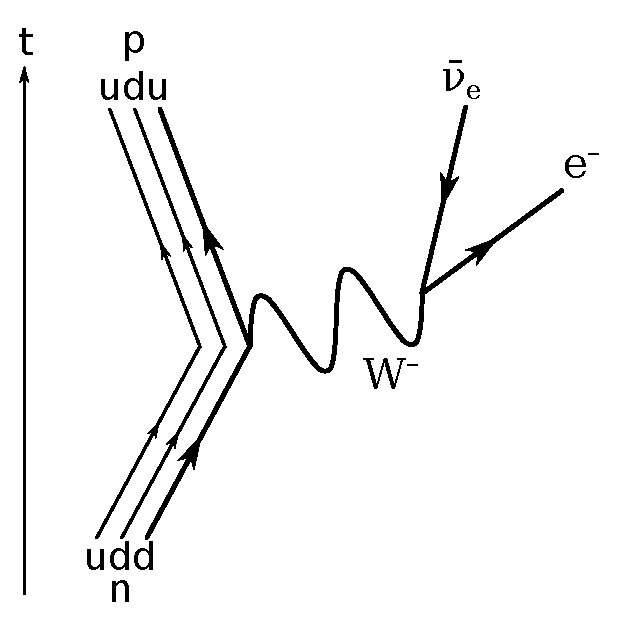
\includegraphics[width=0.3 \textwidth]{figures/beta_negative_decay.pdf}
    \caption[The leading order Feynman diagram of free neutron $\beta$ decay]
    {The leading order  Feynman diagram of free neutron $\beta$ decay. Image from \cite{beta_decay_fig}}
    \label{fig:beta_decay}
\end{figure}

Free neutrons undergo $\beta$ decay
%
\begin{gather}
    \text{n}\rightarrow \text{p}+ e^-+\bar{\nu}_e
\end{gather}
%
governed by the neutron lifetime (decay time) $\gls{tau_n}=\glsvalue*{tau_n}$ \cite{pdg2022}. The Feynman diagram to leading order for this process is given in Fig.~\ref{fig:beta_decay}. The neutron lifetime designates the amount of helium created during Big Bang nucleosynthesis. The CKM matrix element $V_\text{ud}$ (Eq.~\ref{eq:CKM}) can be determined from measurements of \gls{tau_n} in combination with measurements of $0^+\rightarrow0^+$ decays~\cite{Young2014}.

The most accurate neutron lifetime experiments to date have been storage experiments with \ucn held by magnetic and gravitational potentials, such as the UCN$\tau$ experiment at \acrshort{lanl} \cite{gonzalez_ucn_tau}. There is an ongoing disagreement between neutron lifetime storage experiments that count surviving \ucn and neutron lifetime cold beam experiments that count the proton decay products~\cite{czarnecki2018}.

The neutron beta decay directional distribution and total decay rate can be very generally written in terms of the neutron spin and lepton momenta by the expression~\cite{Young2014}
%
\begin{align}
    d\Gamma(\vv{p}_e, \vv{p}_{\bar{\nu}}) &= dE_e\,d\Omega_e \,d\Omega_{\bar{\nu}} \frac{F(E_e)\,p_e E_e (E_o-E_e)^2}{(2\pi)^5} \xi \nonumber \\
    &\quad\quad \times \left[1 + a\frac{\vv{p}_e \cdot \vv{p}_{\bar{\nu}}}{E_e E_{\bar{\nu}}}
    +b\frac{m_e}{E_e} + \langle \vv{S}_\text{n} \rangle \cdot
    \left( A\frac{\vv{p}_e}{E_e} + B \frac{\vv{p}_{\bar{\nu}}}{E_e} + D\frac{\vv{p}_e\times \vv{p}_{\bar{\nu}}}{E_e E_{\bar{\nu}}}
    \right) \right]
\end{align}
%
$\vv{S}_\text{n}$ is neutron spin, $F(E_e)$ is the Fermi function for final state interactions, $E_o$ is the endpoint energy, $E_e$ and $\vv{p}_e$ are electron energy and momentum, and $E_{\bar{\nu}}$ and $\vv{p}_{\bar{\nu}}$ are anti-neutrino energy and momentum.

Of interest are correlation coefficients $a$, $b$, $A$, $B$, and $D$, which are experimental observables. Measurements of these coefficients are a probe of the V\textendash A structure of the \acrshort{sm}. 
%
\begin{itemize}
    \item Electron-antineutrino asymmetry $a$ is measured from the proton spectrum.
    \item Fierz interference coefficient $b$ is measured from the $\beta$ spectrum. $b$ is nominally $0$ in the \acrshort*{sm}.
    \item Beta asymmetry $A$ is determined from the angular correlation between the emitted electron and neutron polarization.
    \item Spin-antineutrino asymmetry $B$ is found via the angular correlation of the recoil proton and neutron polarization.
    \item Triple product $D$ arises from the triple correlation between electron momentum, proton momentum, and neutron spin. $D$ is also nominally $0$ in the \acrshort*{sm}.
\end{itemize}

Reference~\cite{Young2014} provides a review of the $\beta$ decay experimental program at \acrshort{lanl}. (In this section we followed conventional notation for $\beta$ decay observables, but variables $a$, $b$, $A$, $B$, and $D$ will be used to denote other parameters for the remainder of this dissertation.) 


%%%%%%%%%%%%%%%%%%%%%%%%%%%%%%%%%%%%%%%%%

\section{Strong interaction}

%%%%%%%%%%%%%%%%%%%%%%%%%%%%%%%%%%%%%%%%%

Neutrons and protons are bound in nuclei via the strong interaction. In the low energy limit the strong force between the proton and neutron can be approximated by attractive square-well potential of depth \qty{40}{\mega\eV} with radius $2\times10^{-5}\text{ m}$. A more accurate representation is the Fermi potential, a square well with rounded corners. This Fermi potential is not to be confused with the optical potential, also proposed by Fermi, described in Sec.~\ref{sec:ucn_matter_int}. The force between a neutron and a nucleus is also approximated by a square well with $r=r_0A_m^{1/3}$ for mass number $A_m$ and the constant $r_0=1.2\times10^{-15}\text{ m}$ \cite{golubUCN}.

Neutrons may be absorbed (captured) by nuclei. When absorbed, a $\gamma$ ray or charged particle ($[\text{n},\text{p}]$ or $[\text{n},\alpha]$) is released. Absorption cross sections are further discussed in Sec.~\ref{sec:ucn_absorption}.

%%%%%%%%%%%%%%%%%%%%%%%%%%%%%%%%%%%%%%%%%

\section{UCN interactions with matter}\label{sec:ucn_matter_int}

%%%%%%%%%%%%%%%%%%%%%%%%%%%%%%%%%%%%%%%%%

Chapter 2 of Ref.~\cite{golubUCN} provides a very thorough description of neutron interactions with matter. The interaction of \ucn with some material is given by a complex ``optical potential,'' or ``pseudo-potential,'' of the form
%
\begin{gather}
    U = V - iW = \frac{2\pi\hbar^2}{\gls{m_n}}\gls*{rho_N} b_\text{c}-i\frac{\hbar}{2}\gls*{rho_N} \sigma_{\text{t}} v \label{eq:optical_potential}
\end{gather}
%
where \gls{m_n} is the neutron mass, $v$ is the velocity of the neutron, $b_\text{c}$ is the coherent neutron scattering length of the material, $\sigma_{\text{t}}$ is the total loss cross section, and $\gls*{rho_N}$ is number density. Number density can be expressed in units~[\unit{\meter^{-3}}] by the relation $\gls*{rho_N}=\rho_\text{mat}N_A/w_\text{at}$, where $\rho_\text{mat}$ [\unit{\g\per\m^3}] is material density, $w_\text{at}$ [\unit{\g\per\mole}] is atomic weight, and $N_A$ [\unit{\mole^{-1}}] is Avogadro's number.

The real component of optical potential $V$ describes the critical neutron energy that may be confined by a material, and the imaginary part $W$ describes absorption and upscattering within the material. Table~\ref{tb:optical_potentials} lists the UCN optical potentials of commonly used materials in nEDM experiments.

\begin{table}
\centering
\caption[UCN optical potentials of selected UCN materials. V is the real component and W is the imaginary component]{\label{tb:optical_potentials}UCN optical potentials of selected materials. $V$ is the real component and $W$ is the imaginary component.}
\begin{tabular}{
    l
    l
    S[table-format = 3.1]
    S[exponent-mode = scientific, table-format = 2.3e1]
    c
}
\toprule
Material & Abbrv. & {V [\unit{\nano\eV}]} & {W [\unit{\nano\eV}]} & Ref.\\ 
\midrule
Aluminum & Al & 54.1 & 0.00281 & \cite{atchison_transmission_2009}\\
Copper & Cu & 168 & 0.0252 & \cite{golubUCN}\\
Diamond-like carbon & \acrshort{dlc} & 250 & 0.0875 & \cite{Atchison2006} \\
Deuterated polystyrene & \acrshort{dps} & 161 & 0.0483 & \cite{bodek_storage_2008} \\
$\ce{^{58}}\text{Nickel}$ & $\ce{^{58}Ni}$ & 335 & 0.0503 & \cite{golubUCN} \\
Nickel Molybdenum & \acrshort{nimo} & 221.5 & 0.027 & \cite{bondar_losses_2017}  \\
Nickel Phosphorus & \acrshort{nip} & 213 & 2.3e-2 & \cite{pattie_jr_evaluation_2017}  \\
Stainless Steel & \acrshort{ss} & 183 & 0.055 & \cite{akatsuka_characterization_2023} \\
\bottomrule
\end{tabular}
\end{table}

%%%%%%%%%%%%%%%%%%%%%%%%%%%%%%%%%%%%%%%%%

\subsection{Reflection and transmission}\label{sec:ucn_reflection_transmission}

%%%%%%%%%%%%%%%%%%%%%%%%%%%%%%%%%%%%%%%%%

Consider a neutron traveling in a material of potential $V$, with kinetic energy $K$. Let the neutron be incident on a second material of potential $V'$ and imaginary potential $W$, with an energy component perpendicular to the surface of the second material $K_\perp$. The incident neutron may be treated as a propagating wave function $\psi = \exp (ikx)$ with wave vector $k=\sqrt{2\gls{m_n}K/\hbar^2}$.

Reflection probability $R$ arises from continuity requirements at the incidence boundary, and is given by~\cite{golubUCN, schreyer_thesis}
%
\begin{gather}
    R = \begin{cases}
        \left| \frac{\sqrt{K_\perp}-\sqrt{K_\perp - (V'-V)}}{\sqrt{K_\perp} + \sqrt{K_\perp - (V'-V)}}\right|^2 \quad \text{for } K_\perp > (V'-V) \\
        \left| \frac{\sqrt{K_\perp}-\sqrt{K_\perp - (V'-V) + iW}}{\sqrt{K_\perp} + \sqrt{K_\perp - (V'-V) + iW}} \right|^2 \quad \text{for } K_\perp < (V'-V) \label{eq:loss_on_reflection}
    \end{cases}
\end{gather}
%
Under the condition $K_\perp < (V'-V)$, the neutron cannot be transmitted, only reflected. However, as per Eq.~\ref{eq:loss_on_reflection}, there is a reflection loss probability. The wave function of a reflected \ucn penetrates a small distance into the incidence surface, where it may be lost by the interactions described in Sec.~\ref{sec:ucn_absorption}.

If $K_\perp > (V'-V)$ and the neutron is not reflected, it undergoes refraction and is transmitted through the surface into the second material. The energy of the neutron within the second material is given by $K'=K-(V'-V)$. The refraction is analogous to Snell's law, where the velocity component in the first material perpendicular to the refraction surface $v_\perp$ is changed and the component parallel to the surface $v_\parallel$ is unaltered. The velocity in the second material $v'$ is given by
%
\begin{align}
    \vv{v}' &= \vv{v}_\parallel+ \vv{v}'_\perp \\
    &= \vv{v}_\parallel + \left( \sqrt{\frac{K_\perp}{K_\perp - (V'-V)}} \right)\vv{v}_\perp \\
    &= \vv{v} + \left( \sqrt{\frac{K_\perp}{K_\perp - (V'-V)}} - 1 \right)\vv{v}_\perp
\end{align}

%%%%%%%%%%%%%%%%%%%%%%%%%%%%%%%%%%%%%%%%%

\subsection{Absorption and up-scattering}\label{sec:ucn_absorption}

%%%%%%%%%%%%%%%%%%%%%%%%%%%%%%%%%%%%%%%%%

The two main loss mechanisms for \ucn within a material are absorption and inelastic up-scattering. Absorption occurs when the neutron is captured by nuclei, and inelastic upscattering occurs when a thermally vibrating nucleus increases the energy of \ucn such that it may no longer be stored. The total loss cross section $\sigma_{\text{t}}$ (from Eq.~\ref{eq:optical_potential}) is the sum of absorption cross section $\sigma_\text{abs}$ and inelastic up-scattering cross section $\sigma_\text{inel}$.

Absorption cross sections are well quantified (see Ref.~\cite{nist_neutron_cross_sections}), but up-scattering cross sections are mostly unknown. Among many other factors, surface impurities with large inelastic scattering cross sections (e.g. hydrogen, $\sigma_\text{inel} \sim \qty{80}{\barn}$ \cite{nist_neutron_cross_sections}), will heavily affect up-scattering probabilities. When simulating \ucn material interactions it is often easier to make the assumption $\sigma_{\text{t}} \cong \sigma_\text{abs}$, and to treat up-scattering as a separate effective loss per bounce parameter, as described in Sec.~\ref{sec:loss_per_bounce}.

The absorption cross section $\sigma_\text{abs}$ is proportional to $1/v$. From the second term of Eq.~(\ref{eq:optical_potential}) it becomes apparent that $W$ is independent of neutron velocity in the material.

Absorption loss probability may be expressed by non-conservation of current density $\vv{j}$ \cite{golubUCN}
%
\begin{gather}
    \vv{j} = \frac{\hbar}{2m} ( \psi^* \vv{\nabla} \psi - \psi \vv{\nabla}\psi^*)
\end{gather}
%
For some neutron wave function propagating through a material $\psi = \exp (ik'x)$ with wave vector $k'=\sqrt{2m(K'+iW)}/\hbar$. This gives
%
\begin{gather}
    j \propto e^{-2\,\text{Im}(k')x}
\end{gather}
%
The loss probability after traveling is distance $x$ through a material is then
%
\begin{gather}
    P_\text{abs}= 1 - \exp \left[2\,\text{Im}\left( \frac{\sqrt{2m(K'+iW)}}{\hbar}\right)x \right]\label{eq:pentrack_absorption}
\end{gather}
%
Equation~\ref{eq:pentrack_absorption} is the absorption probability calculation utilized in the \ucn simulation software \pentrack~\cite{schreyer_pentrack} (see Chap.~\ref{chap:simulations}). Another equivalent method for quantifying neutron absorption within a material is discussed in Sec.~\ref{sec:beer_lambert_law}.

%%%%%%%%%%%%%%%%%%%%%%%%%%%%%%%%%%%%%%%%%

\subsection{Loss per bounce}\label{sec:loss_per_bounce}

%%%%%%%%%%%%%%%%%%%%%%%%%%%%%%%%%%%%%%%%%

The average loss probability per bounce $\bar{\mu}(K)$ for a \ucn of kinetic energy $K$ is obtained by assuming ideal gas conditions and averaging loss per bounce over all angles of incidence. Equation~(2.70) in Ref.~\cite{golubUCN} gives
%
\begin{gather}
    \bar{\mu} = 2f \left[ \frac{V}{K} \sin^{-1}\left( \frac{K}{V}\right)^{1/2} -\left( \frac{V}{K} - 1 \right)^{1/2} \right] \label{eq:lossPerBounce_golub}
\end{gather}
%
The loss factor is $f=W/V$, for optical potential terms $V$ and $W$ from Eq.~(\ref{eq:optical_potential}). For a more phenomenological treatment of loss per bounce, Eq.~(\ref{eq:lossPerBounce_golub}) may be modified by replacing $f$ with a free parameter $\mu$, a velocity independent effective loss per bounce. See Secs.~\ref{subsec:storageCurves} and \ref{sec:1D_random_walk} for example applications.

%%%%%%%%%%%%%%%%%%%%%%%%%%%%%%%%%%%%%%%%%

\subsection{Beer-Lambert Law}\label{sec:beer_lambert_law}

%%%%%%%%%%%%%%%%%%%%%%%%%%%%%%%%%%%%%%%%%

Neutron flux attenuation after passing through material can be described with the Beer-Lambert law. Here we model neutron absorption and elastic scattering within material.

Let a beam of neutrons be incident on a material with area $A$, thickness $dx$, and density of atoms (number density) $\gls*{rho_N}$. The number of atoms hit by the incident beam of intensity $I$ is given by $\gls*{rho_N} A\,dx$. The ``effective area'' of the atoms is given by $\sigma \gls*{rho_N} A \, dx$, where $\sigma$ is an absorption or scattering cross section of neutrons on the material.

Therefore, the probability of the a neutron being absorbed or scattered out of the beam in a material of thickness $dx$ is given by
%
\begin{gather}
    -\frac{dI}{I}=\frac{\sigma\gls*{rho_N} A}{A}dx
\end{gather}
%
where $dI$ is the change in intensity as the beam traverses the distance $dx$. Integrating both sides of the equation gives
%
\begin{align}
    \int^I_{I_0}\frac{dI}{I} &= -\int^x_0 \sigma \gls*{rho_N} \,dx \\
    \frac{I}{I_0} &= \exp(-\sigma \gls*{rho_N} x) \label{eq:beer_lambert_law_variant}
\end{align}
%
Where $I_0$ is the beam density intensity at the entrance of the material. Defining the mean free path inside the material as $\lambda_\text{mfp}=1/(\gls*{rho_N} \sigma)$ we get the Beer-Lambert law, which describes flux attenuation.
%
\begin{gather}
    I(x) = I_0 \exp(-x/\lambda_\text{mfp}) \label{eq:beer_lambert_law}
\end{gather}
%
 The Beer-Lambert law applies to neutrons, photons, and rarefied gases. See Appx.~\ref{appx:199hg_pumping} for an example application to the \qty{254}{\nano\meter} laser used for optical pumping of the $\ce{^199Hg}$ comagnetometer. 
 
 We consider the process of bulk elastic scattering, when the neutron collides with the material and has its trajectory altered according to a Lambertian distribution. The probability $P_\text{elastic}$ after traversing a distance $x$ through a material is given by
%
\begin{gather}
    P_\text{elastic}=1-\exp(-x \gls*{rho_N} \sigma_\text{inc})
\end{gather}
%
where $\sigma_\text{inc}$ is the incoherent cross section for thermal neutrons (see Ref.~\cite{nist_neutron_cross_sections}). Similarly, the chance for absorption in a material for a \ucn with velocity $v$ may be described by
%
\begin{gather}
    P_\text{abs}= 1-\exp(-x \gls*{rho_N} \sigma_\text{abs}v_\text{thermal}/v)
\end{gather}
%
where $\sigma_\text{abs}$ is the absorption cross section for thermal neutrons ($v_\text{thermal}=\qty{2200}{\meter\per \s}$) as listed in Ref.~\cite{nist_neutron_cross_sections}.

%%%%%%%%%%%%%%%%%%%%%%%%%%%%%%%%%%%%%%%%%

\subsection{Diffuse reflections}\label{sec:diffuse_reflections}

%%%%%%%%%%%%%%%%%%%%%%%%%%%%%%%%%%%%%%%%%

\begin{figure}
\centering
%subfigure width gets "multiplied" by includegraphics width
\begin{subfigure}{.5\textwidth} 
  \centering
  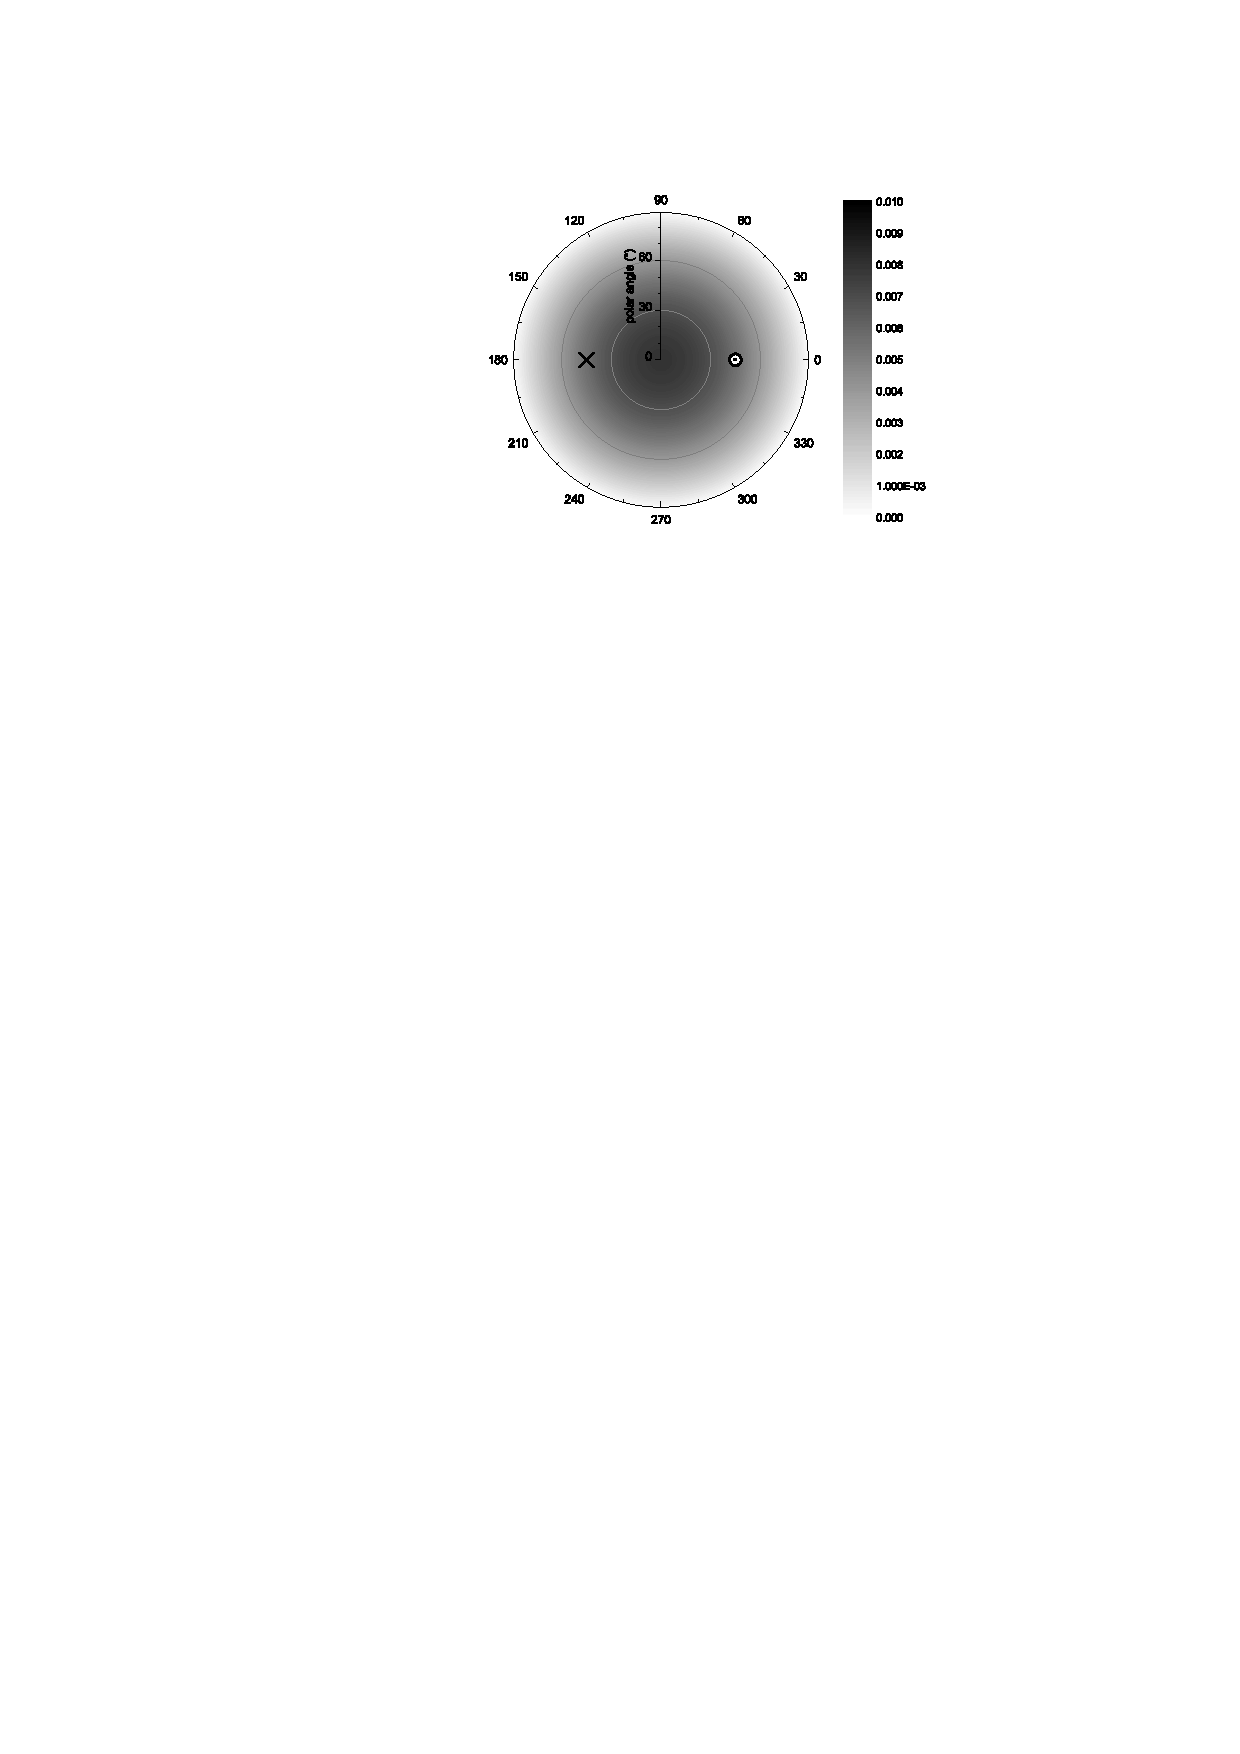
\includegraphics[width=\textwidth]{figures/schreyer_lambertian.pdf}
  \caption{Lambert ($\cos\theta$) distribution}\label{subfig:lambert_diffuse}
\end{subfigure}%DO NOT REMOVE THIS '%'
\begin{subfigure}{.5\textwidth}
  \centering
  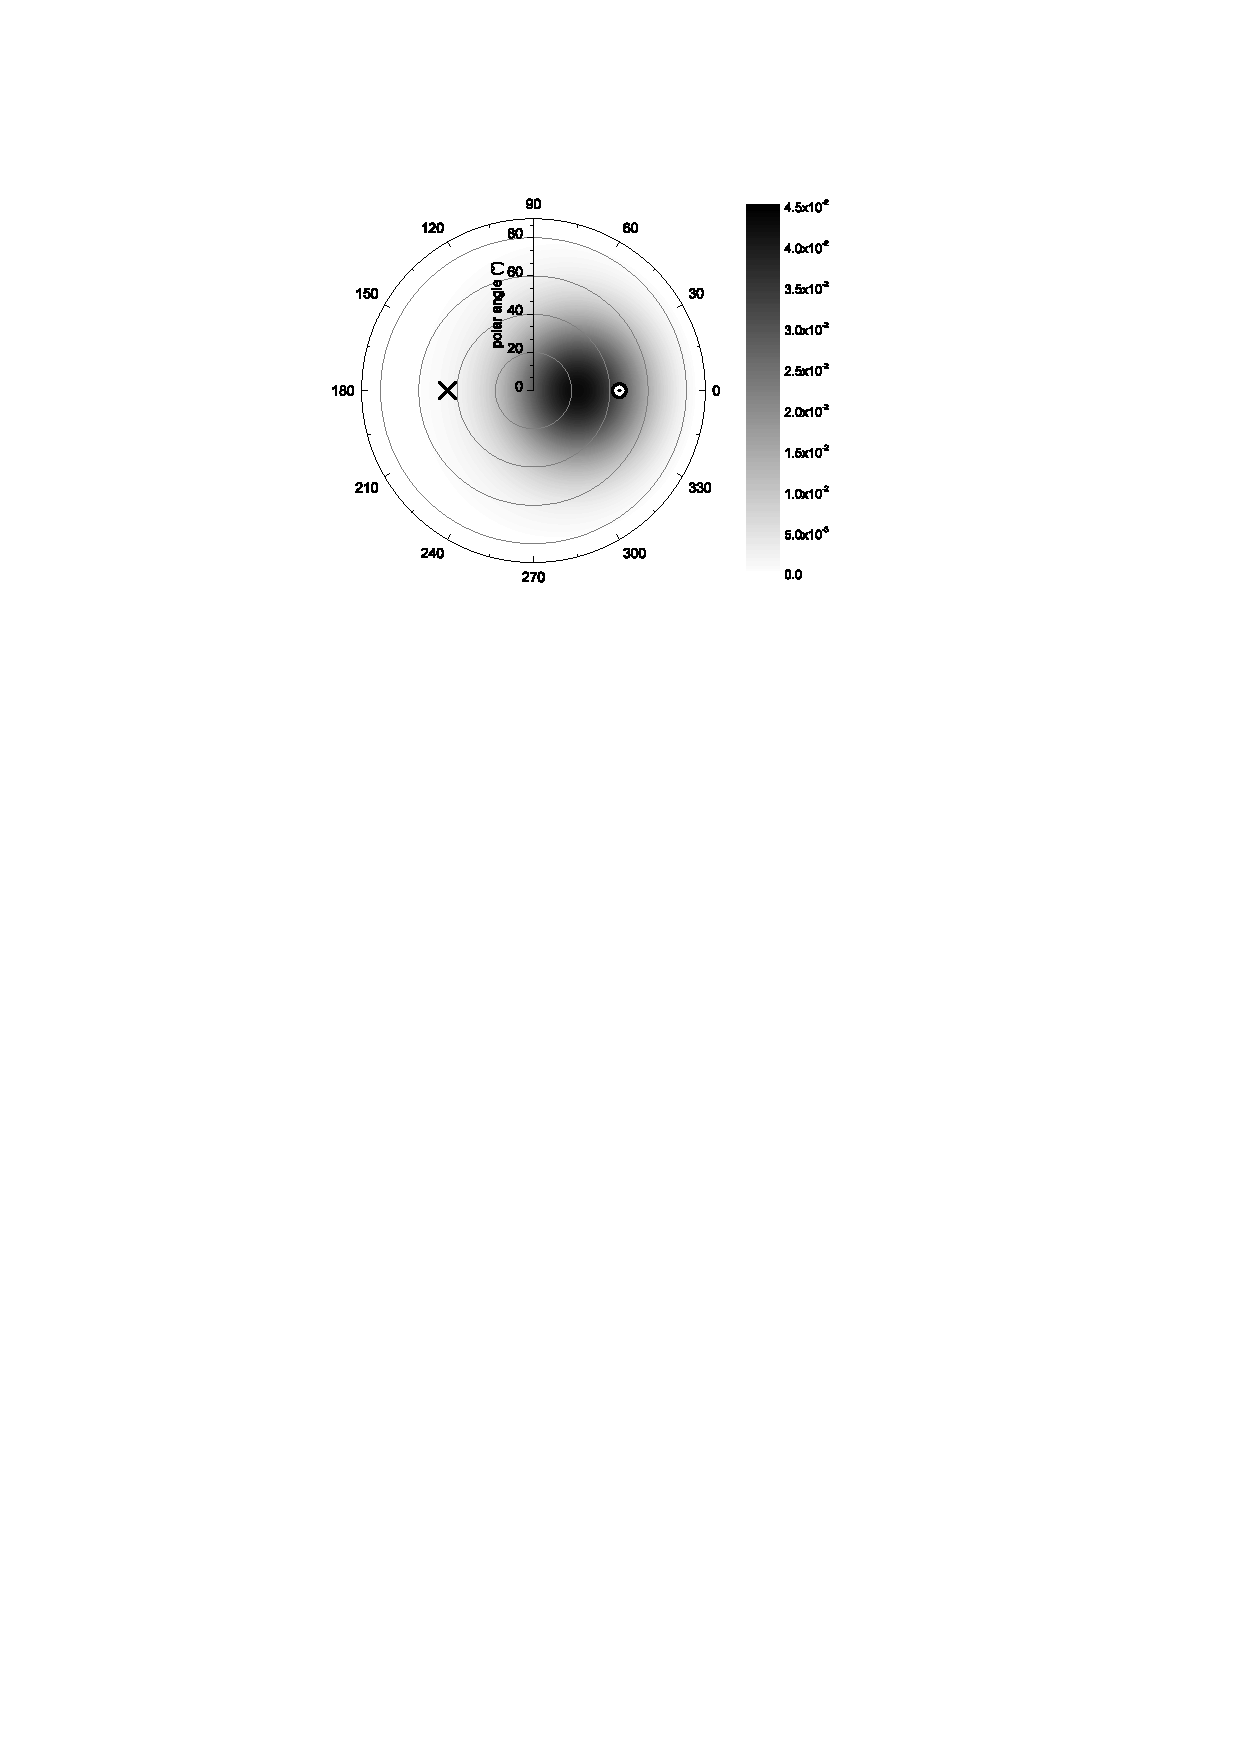
\includegraphics[width=\textwidth]{figures/schreyer_microroughness.pdf}
  \caption{Micro-roughness}\label{subfig:microroughness_diffuse}
\end{subfigure}
\caption[Two types of diffuse reflection]
{Two types of diffuse reflection. Images from Ref.~\cite{schreyer_thesis}. The cross is the incoming direction of the \ucn (\qty{45}{\degree}) and the dot is the direction of specular reflection. \textbf{(a)} Intensity of Lambertian reflection from Eq.~(\ref{eq:lambertian_reflection}) ($P_\text{L}=0.05$). \textbf{(b)} Intensity of micro-roughness reflection on \acrshort{ss} ($K=\qty{150}{\nano\eV}$, $V=\qty{183}{\nano\eV}$, $b_\text{MR}=\qty{2.5}{\nano\meter}$, $w_\text{MR}=\qty{20}{\nano\meter}$, $P_\text{MR}=\qty{4.9}{\percent}$)}
\label{fig:diffuse_reflection}
\end{figure}


\ucn incident on a smooth surface are usually reflected specularly, such that the angle of incidence is equal to the angle of reflection. However, there is a small material-dependent chance ($\sim\qtyrange{1}{10}{\percent}$) of diffuse (nonspecular) reflection. Diffusivity also affects the trajectory of refracted 
\ucn during transmission through a surface. The simplest version of diffuse reflection uses a Lambertian, or $\cos\theta$, distribution to determine the reflected intensity
%
\begin{gather}
    I_\text{L}(\theta)d\Omega=\frac{P_\text{L}}{\pi}\cos\theta\,d\Omega\label{eq:lambertian_reflection}
\end{gather}
%
where $P_\text{L}$ is some fixed probability of diffuse reflection and $d\Omega$ is the solid angle. The parameter $\theta$ has a range $[0,\pi/2]$. Lambertian reflection has no dependence on the angle of incidence (see Fig.~\ref{subfig:lambert_diffuse}).

A more accurate model of diffuse reflection is micro-roughness. A material surface is treated as a smooth plane with a perturbation, which causes diffuse scattering through diffraction and interference. Reference~\cite{atchison_diffuse_2010} experimentally validates the model described in Refs.~\cite{steyerl_1972, steyerl_surface_2010}, and an example of micro-roughness implementation in \ucn simulations is found in \pentrack~\cite{schreyer_pentrack}. Micro-roughness is characterized by surface roughness amplitude $b_\text{MR}$ and correlation length $w_\text{MR}$. For incident angle $\theta_\text{i}$ ($\phi_\text{i}=0$) and outgoing angles $\theta_\text{f}$, $\phi_\text{f}=0$, the reflection intensity $I_\text{R}$ and transmission intensity $I_\text{T}$ are given by~\cite{steyerl_1972, schreyer_thesis}
%
\begin{gather}
    \begin{align}
        I_\text{R}(k, \theta_\text{i}, \theta_\text{f}, \phi_\text{f})\,d\Omega_\text{f} &=  |S(\theta_\text{i})|^2|S(\theta_\text{f})|^2 F(k,\theta_\text{i}, \theta_\text{f}, \phi_\text{f})\,d\Omega_\text{f} \\
        I_\text{T}(k, k', \theta_\text{i}, \theta_\text{f}, \phi_\text{f})\,d\Omega_\text{f} &=  \frac{k'}{k}|S(\theta_\text{i})|^2|S(\theta_\text{f})|^2 F(k,\theta_\text{i}, \theta_\text{f}, \phi_\text{f})\,d\Omega_\text{f} \\
        S(\theta,k) &= \frac{2\cos\theta}{\cos\theta+\sqrt{\cos^2\theta-k_\text{c}/k}}
    \end{align}\\
    F(k,\theta_\text{i}, \theta_\text{f}, \phi_\text{f}) = \frac{k^4_\text{c}(b_\text{MR}w_\text{MR})^2}{8\pi\cos\theta_\text{i}} \exp \left[-\frac{(w_\text{MR}k)^2}{2} (\sin^2\theta_\text{i}+\sin^2\theta_\text{f} - 2\sin\theta_\text{i}\sin\theta_\text{f}\cos\phi_\text{f})\right]
\end{gather}
%
where following the notation from Sec.~\ref{sec:ucn_reflection_transmission}, the incident \ucn wave vector is $k=\sqrt{2\gls{m_n}K/\hbar^2}$, the transmitted wave vector is $k'=\sqrt{2\gls{m_n}(K - (V'-V))/\hbar^2}$, and the critical wave vector for total reflection is $k=\sqrt{2\gls{m_n}(V'-V)/\hbar^2}$.

Unlike Lambertian reflection, the probability of micro-roughness reflection or transmission is not a free parameter, and is given by
%
\begin{gather}
    P_\text{MR}=\int_{2\pi} I_\text{R,T}(k, \theta_\text{i}, \theta_\text{f}, \phi_\text{f})\,d\Omega_\text{i}=\int_0^{\pi/2}d\theta_\text{f}\int_0^{2\pi}d\phi_\text{f}\,I_\text{R,T}(k, \theta_\text{i}, \theta_\text{f}, \phi_\text{f})
\end{gather}
%
Fig.~\ref{subfig:microroughness_diffuse} shows an example of diffuse reflection using micro-roughness.